%==============================================================================
% Voorbeeld hogent-article: onderzoeksvoorstel bachproef
%==============================================================================

\documentclass{hogent-article}

% Invoegen bibliografiebestand
\addbibresource{bronnen.bib}

% Informatie over de opleiding, het vak en soort opdracht
\studyprogramme{Professionele bachelor toegepaste informatica}
\course{Bachelorproef}
\assignmenttype{Onderzoeksvoorstel}
\academicyear{2023-2024}

\title{Heeft de maancyclus een invloed op het gedrag van de cryptocurrency markt?: een onderzoek naar een correlatie tussen de maancyclus en de cryptomarkt door gebruik te maken van AI}

\author{Hanno van Baarle}
\email{hanno.vanbaarle@student.hogent.be}

% Gaat het om een bachelorproef in samenwerking met een student in een andere
% opleiding? Geef dan de naam en emailadres hier
% \author{/}
% \email{/}

% TODO: Geef de co-promotor op
%\supervisor[Co-promotor]{S. Beekman (Synalco, \href{mailto:sigrid.beekman@synalco.be}{sigrid.beekman@synalco.be})}

% Binnen welke specialisatierichting uit 3TI situeert dit onderzoek zich?
% Kies uit deze lijst:
%
% - Mobile \& Enterprise development
% - AI \& Data Engineering
% - Functional \& Business Analysis
% - System \& Network Administrator
% - Mainframe Expert
% - Als het onderzoek niet past binnen een van deze domeinen specifieer je deze
%   zelf
%
\specialisation{AI \& Data Science}
\keywords{AI, Cryptocurrency, Blockchain, Mooncycles, Financiën}

\begin{document}

\begin{abstract}
    In dit onderzoeksvoorstel wordt de potentiële correlatie tussen de maancyclus en de cryptocurrency markt onderzocht, met behulp van geavanceerde artificiële intelligentie (AI) en machine learning-algoritmen. De studie richt zich op het analyseren van een breed scala aan parameters, waaronder prijsbewegingen, handelsvolume, de 'greed-index', en Bitcoin-dominantie. De literatuurstudie belicht eerdere onderzoeken, waaronder studies die zowel correlaties als tegenstrijdige bevindingen hebben gepresenteerd. De methodologie omvat de verzameling van maancyclus en cryptocurrency data, gevolgd door samenvoeging, data cleaning, modeltraining, en fine-tuning. Het verwachte resultaat is een diepgaand inzicht in mogelijke correlaties, met een nadruk op het aantonen of weerleggen van de invloed van de maancyclus op de cryptocurrency markt. Het rapporteren en documenteren van het onderzoeksproces, samen met een Gantt chart, vervolledigen dit onderzoeksvoorstel.
\end{abstract}

\tableofcontents

\section{Inleiding}%
\label{sec:inleiding}

In de snel evoluerende wereld van cryptocurrency's wordt gezocht naar innovatieve benaderingen om het gedrag van de markt beter te begrijpen en voorspellingen te verbeteren. Een ongewoon doch intrigerend aspect dat de aandacht heeft getrokken, is de maancyclus. Dit onderzoek tracht te onderzoeken of er al dan niet een aantoonbare correlatie bestaat tussen de verschillende fasen van de maancyclus en het gedrag van de cryptomarkt.

De maancyclus, die zich over een periode van ongeveer 29,5 dagen voltrekt, heeft eeuwenlang fascinatie gewekt en is vaak in verband gebracht met diverse aspecten van het menselijk leven en de natuur. Zo was de maan bijvoorbeeld een teken van tijd, vruchtbaarheid en groei in het oude Egypte \textbf{\cite{MoonCraterTycho2023}}. Dit onderzoek gaat een stap verder door gebruik te maken van geavanceerde artificiële intelligentie (AI) om patronen te identificeren en mogelijke correlaties tussen de maancyclus en de cryptomarkt te analyseren.

Door middel van geautomatiseerde data-analyse, machine learning-algoritmen en diepgaande marktgegevens, beoogt dit onderzoek niet alleen de aanwezigheid van correlaties te identificeren, maar ook inzichten te krijgen in hoe dergelijke cyclische patronen invloed zouden kunnen hebben op het gedrag van de cryptomarkt. Dit zou niet alleen van academisch belang kunnen zijn, maar ook praktische implicaties kunnen hebben voor beleggers en marktdeelnemers die trachten de volatiliteit van cryptocurrency's beter te begrijpen en te benutten.

Voorgaande studies hebben reeds onderzoek gedaan naar de potentiële invloed van de maan op zowel de aandelen- als de cryptomarkt. Echter, deze studies concentreerden zich specifiek op de prijsbewegingen van individuele aandelen of cryptocurrencies en verkenden niet de bredere marktinvloeden. Het onderscheidende kenmerk van deze studie ligt in haar streven om verder te gaan dan enkel prijsanalyses. In plaats daarvan richt deze studie zich op een uitgebreidere reeks parameters, waaronder handelsvolume (TV), de 'greed-index', en Bitcoin-dominantie. Door deze brede benadering beoogt de studie niet alleen de invloed van de maan op prijzen te onderzoeken, maar ook op de algehele marktdynamiek. Dit streven naar een meer omvattende analyse positioneert deze studie als een unieke bijdrage aan het bestaande onderzoek op het raakvlak van maancycli en financiële markten.

\section{Literatuurstudie}%
\label{sec:Literatuurstudie}

ookal heeft de studie een focus op de volledige markt blijft het waardevol om eerdere studies met betrekking tot specifieke cryptocurrencies, zoals Bitcoin en andere `digital currencies`, grondig te onderzoeken. 
\newline

In 2023 deden 4 studenten aan de universiteit van Hacettepe, Ugurcan Erdogan, Alperen Berk Isildar, Tugba Gurgen Erdogan en Fuat Akal \textbf{\textcite{Lunarcycles2023}} een studie rond de prijs impact van lunar cycles op bitcoin. Ze maakten hier gebruik van McNemar's Chi-Square test om onderzoek te doen. In hun studie concludeerden de studenten dat er volgens de Chi-Square test hoogstwaarschijnlijk geen duidelijk correlatie is tussen de prijs van Bitcoin en de cycli van de maan.
\newline

Een andere studie in 2014 vond een tegenstrijdige conclusie waaruit bleek dat beleggerspsychologie wordt beïnvloed door de volle maan, er werden echter geen effecten waargenomen tijdens de nieuwe maanfase. Bevestigd door de paired t-difference test, de kleine correlatie, naast het kwantitatieve model, tonen de resultaten aan dat de volle maan invloed heeft op het marktgedrag tijdens haar `orbital phase`. Als gevolg hiervan veronderstellen de auteurs dat de volle maan daadwerkelijk van invloed is op de cognitie van beleggers en emotionele verstoring, stemmingsstoornissen en agressiviteit, wat resulteert in een slechte prestatie bij het handelen in aandelen.
\textbf{\textcite{Brahmana2014}}
De studie focust zich voornamelijk op het vinden van psychologische redenen door de maan die dan ook een invloed kunnen hebben op het gedrag van traders.
\newline

In 2013 vonden twee studenten aan Krea university bewijs dat er een duidelijke correlatie is tussen de mooncycli en de stockmarkt.
`We employ recent data from 59 international emerging and mature stock markets to provide new evidence of a lunar cycle (full and new moon) effect on their stock market returns. Using a threshold generalised autoregressive conditional heteroscedasticity (TGARCH) model, we further examine the linkages between efficient-market theory, calendar-related effects and investors’ mood resulting from moon phases. The empirical results show significant full moon effects in six markets, and significant new moon effects in eight markets`
\textbf{\cite{Floros2013}}
Ze vonden echter ook dat deze correlatie sterk samenvalt met de `calender anomalies`:
\newline
`In addition, we find that lunar effects are strongly influenced by the calendar anomalies (Monday effect and January effect)`



\section{Methodologie}%
\label{sec:Methodologie}

\subsection{Voorbereiding}
De voorbereiding fase omvat het aanvragen van een Binance API key voor de cryptocurrency Data
en het opzoek gaan naar een gepaste dataset voor Maancyclus data. Binance is de grootste cryptocurrency exchange waar meer dan 100miljoen traders elke dag gebruik van maken. \textbf{\textcite{Binance©2023}}

\subsection{Verzamel Maancyclus Data}
Zowel de Maancyclus als de cryptocurrency data zal tegelijk verzameld worden. Deze studie zal zich focussen op \textbf{Data van 2022 tot het heden}. De deliverable voor deze fase is een CSV met maancyclus data.

\subsection{Verzamel Cryptocurrency Data}
Deze fase verloopt parallel met de vorige fase. Het betreft niet enkel om de prijs van verschillende cryptocurrencies maar ook het totale trading volume (TV) en verschillende andere parameters. De deliverable is ook een CSV met Cryptocurrency data.

\subsection{Samenvoegen}
Na het zorgvuldig verzamelen van de maancyclus data en cryptocurrency marktgegevens, gaan we nu over naar de cruciale fase van het samenvoegen van deze datasets. In deze fase integreren we de maancyclus data met de cryptocurrency gegevens om een holistisch beeld te verkrijgen van mogelijke correlaties tussen deze variabelen.

Het samenvoegen vereist een nauwgezette aanpak, waarbij we de tijdreeksen van beide datasets harmoniseren en de frequentie van de gegevens afstemmen. Door deze zorgvuldige aanpak streven we ernaar om een consistent en representatief kader te creëren voor het identificeren van correlaties tussen de maancyclus en de cryptocurrency markt.
Deze fase heeft als eind delivarable een \textbf{UML diagram} om de relaties tussen verschillende data beter te kunnen begrijpen.

\subsection{Data Cleaning}
Hier voeren we een grondige datacleaning uit om ervoor te zorgen dat de verzamelde gegevens betrouwbaar en consistent zijn. Dit omvat het omgaan met ontbrekende waarden, het identificeren van outliers en het normaliseren van de datasets.

\subsection{Model Training} 
We gebruiken verschillende methodes en machine learning algoritmen om te vergelijken welke beter presteren. Hierbij integreren we de maancyclus data en cryptocurrency gegevens om patronen te ontdekken die wijzen op mogelijke correlaties. De Algoritmes en testen, zoals de Chi-Squared test, worden geselecteerd op het al dan niet kunnen aantonen van correlaties.
Deze fase heeft een werkend/werkende AI modellen als deliverable.

\subsection{Fine-tuning}
Na de initiële modeltraining passen we fine-tuning toe om de nauwkeurigheid en betrouwbaarheid van het model te verbeteren. Dit omvat het aanpassen van parameters en het valideren van het model met verschillende testen.

\subsection{Conclusies Trekken}
Op basis van de huidige resultaten van het getrainde en gefinetunede model trekken we conclusies met betrekking tot de correlaties tussen de maancyclus en de cryptocurrency markt. We identificeren en analyseren momenteel eventuele significante patronen.

\subsection{Rapporteren}
Het rapporteren loopt parallel met het volledige project. bedenkingen, moeilijkheden en obstakels worden zorgvuldig gedocumenteerd in een rapport.

\subsection{Gant Chart}
Ten slotte een Gant chart die de verloop van het project verduidelijkt:

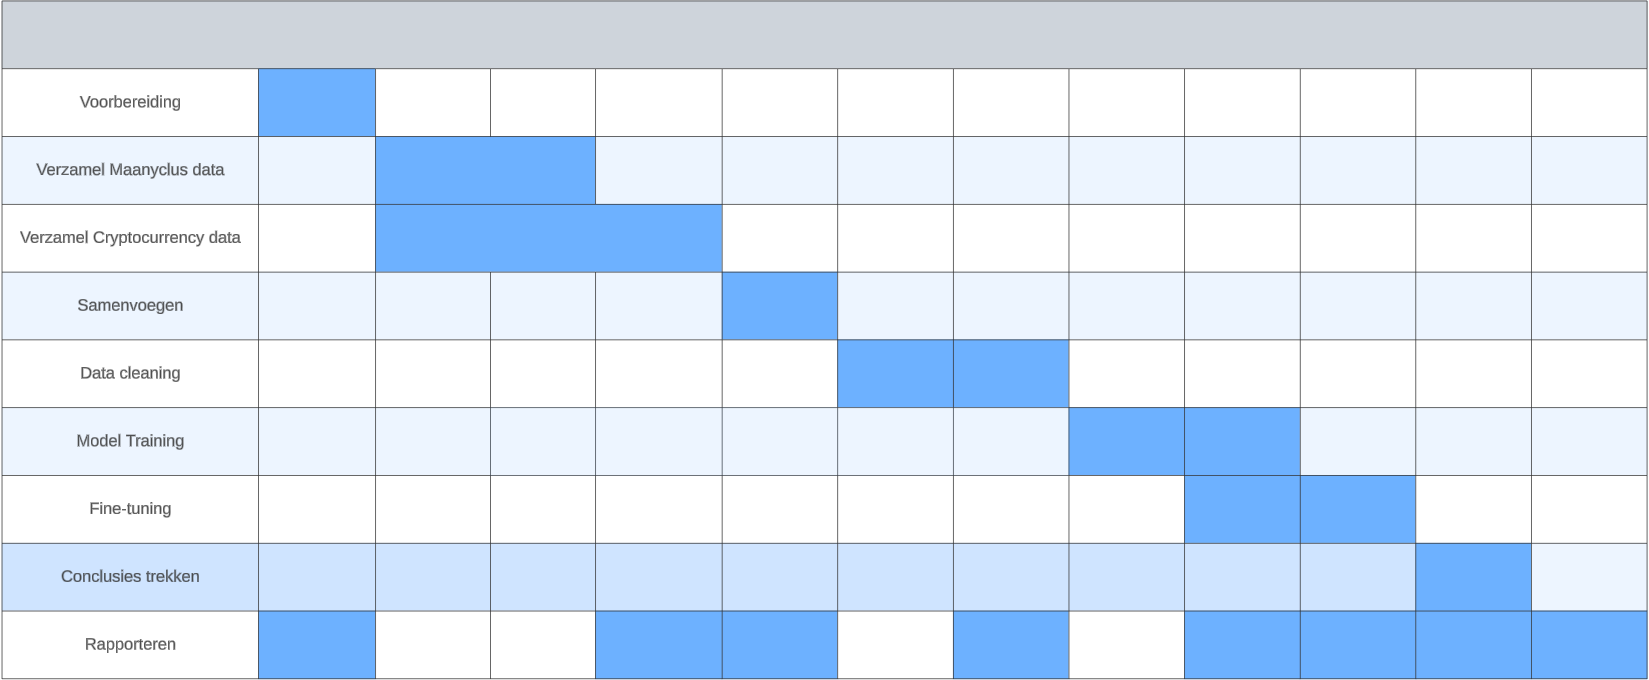
\includegraphics[width=\textwidth]{gantchart.png}

\section{Verwacht resultaat, conclusie}%
\label{sec:Resultaat-en-conclusie}
Alhoewel het idee dat de maancycli invloed hebben op de cryptocurrency markt onrealistisch klinkt is. blijft de academische literatuur hierover verdeeld. Onze hypothese vermoed dat er \textbf{geen meetbare correlatie} is tussen de maan en cryptocurrencies en moesten we toch een meting van correlatie vinden is dit waarschijnlijk te verklaren met de studie van \textbf{\textcite{Brahmana2014}.}

\pagebreak[2]
\printbibliography[heading=bibintoc]

\end{document}